% GNUPLOT: LaTeX picture with Postscript
\begingroup
  \makeatletter
  \providecommand\color[2][]{%
    \GenericError{(gnuplot) \space\space\space\@spaces}{%
      Package color not loaded in conjunction with
      terminal option `colourtext'%
    }{See the gnuplot documentation for explanation.%
    }{Either use 'blacktext' in gnuplot or load the package
      color.sty in LaTeX.}%
    \renewcommand\color[2][]{}%
  }%
  \providecommand\includegraphics[2][]{%
    \GenericError{(gnuplot) \space\space\space\@spaces}{%
      Package graphicx or graphics not loaded%
    }{See the gnuplot documentation for explanation.%
    }{The gnuplot epslatex terminal needs graphicx.sty or graphics.sty.}%
    \renewcommand\includegraphics[2][]{}%
  }%
  \providecommand\rotatebox[2]{#2}%
  \@ifundefined{ifGPcolor}{%
    \newif\ifGPcolor
    \GPcolorfalse
  }{}%
  \@ifundefined{ifGPblacktext}{%
    \newif\ifGPblacktext
    \GPblacktexttrue
  }{}%
  % define a \g@addto@macro without @ in the name:
  \let\gplgaddtomacro\g@addto@macro
  % define empty templates for all commands taking text:
  \gdef\gplbacktext{}%
  \gdef\gplfronttext{}%
  \makeatother
  \ifGPblacktext
    % no textcolor at all
    \def\colorrgb#1{}%
    \def\colorgray#1{}%
  \else
    % gray or color?
    \ifGPcolor
      \def\colorrgb#1{\color[rgb]{#1}}%
      \def\colorgray#1{\color[gray]{#1}}%
      \expandafter\def\csname LTw\endcsname{\color{white}}%
      \expandafter\def\csname LTb\endcsname{\color{black}}%
      \expandafter\def\csname LTa\endcsname{\color{black}}%
      \expandafter\def\csname LT0\endcsname{\color[rgb]{1,0,0}}%
      \expandafter\def\csname LT1\endcsname{\color[rgb]{0,1,0}}%
      \expandafter\def\csname LT2\endcsname{\color[rgb]{0,0,1}}%
      \expandafter\def\csname LT3\endcsname{\color[rgb]{1,0,1}}%
      \expandafter\def\csname LT4\endcsname{\color[rgb]{0,1,1}}%
      \expandafter\def\csname LT5\endcsname{\color[rgb]{1,1,0}}%
      \expandafter\def\csname LT6\endcsname{\color[rgb]{0,0,0}}%
      \expandafter\def\csname LT7\endcsname{\color[rgb]{1,0.3,0}}%
      \expandafter\def\csname LT8\endcsname{\color[rgb]{0.5,0.5,0.5}}%
    \else
      % gray
      \def\colorrgb#1{\color{black}}%
      \def\colorgray#1{\color[gray]{#1}}%
      \expandafter\def\csname LTw\endcsname{\color{white}}%
      \expandafter\def\csname LTb\endcsname{\color{black}}%
      \expandafter\def\csname LTa\endcsname{\color{black}}%
      \expandafter\def\csname LT0\endcsname{\color{black}}%
      \expandafter\def\csname LT1\endcsname{\color{black}}%
      \expandafter\def\csname LT2\endcsname{\color{black}}%
      \expandafter\def\csname LT3\endcsname{\color{black}}%
      \expandafter\def\csname LT4\endcsname{\color{black}}%
      \expandafter\def\csname LT5\endcsname{\color{black}}%
      \expandafter\def\csname LT6\endcsname{\color{black}}%
      \expandafter\def\csname LT7\endcsname{\color{black}}%
      \expandafter\def\csname LT8\endcsname{\color{black}}%
    \fi
  \fi
  \setlength{\unitlength}{0.0500bp}%
  \begin{picture}(9920.00,8332.00)%
    \gplgaddtomacro\gplbacktext{%
      \csname LTb\endcsname%
      \put(726,220){\makebox(0,0)[r]{\strut{} 0}}%
      \put(726,760){\makebox(0,0)[r]{\strut{} 0.5}}%
      \put(726,1299){\makebox(0,0)[r]{\strut{} 1}}%
      \put(858,0){\makebox(0,0){\strut{}}}%
      \put(1917,0){\makebox(0,0){\strut{}}}%
      \put(2976,0){\makebox(0,0){\strut{}}}%
      \put(858,1785){\makebox(0,0)[l]{\strut{}RULE 4: If $x_{1}$ is "$A^{4}_{1}$" AND $x_{2}$ is "$A^{4}_{2}$", then: $y^{(4)}=$linear equation 4}}%
      \put(974,760){\makebox(0,0)[l]{\strut{}$A^{4}_{1}$}}%
    }%
    \gplgaddtomacro\gplfronttext{%
    }%
    \gplgaddtomacro\gplbacktext{%
      \csname LTb\endcsname%
      \put(726,220){\makebox(0,0)[r]{\strut{} 0}}%
      \put(726,760){\makebox(0,0)[r]{\strut{} 0.5}}%
      \put(726,1299){\makebox(0,0)[r]{\strut{} 1}}%
      \put(858,0){\makebox(0,0){\strut{}}}%
      \put(1917,0){\makebox(0,0){\strut{}}}%
      \put(2976,0){\makebox(0,0){\strut{}}}%
      \put(858,1785){\makebox(0,0)[l]{\strut{}RULE 4: If $x_{1}$ is "$A^{4}_{1}$" AND $x_{2}$ is "$A^{4}_{2}$", then: $y^{(4)}=$linear equation 4}}%
      \put(974,760){\makebox(0,0)[l]{\strut{}$A^{4}_{1}$}}%
    }%
    \gplgaddtomacro\gplfronttext{%
    }%
    \gplgaddtomacro\gplbacktext{%
      \csname LTb\endcsname%
      \put(726,220){\makebox(0,0)[r]{\strut{} 0}}%
      \put(726,760){\makebox(0,0)[r]{\strut{} 0.5}}%
      \put(726,1299){\makebox(0,0)[r]{\strut{} 1}}%
      \put(858,0){\makebox(0,0){\strut{}}}%
      \put(1917,0){\makebox(0,0){\strut{}}}%
      \put(2976,0){\makebox(0,0){\strut{}}}%
      \put(858,1785){\makebox(0,0)[l]{\strut{}RULE 4: If $x_{1}$ is "$A^{4}_{1}$" AND $x_{2}$ is "$A^{4}_{2}$", then: $y^{(4)}=$linear equation 4}}%
      \put(974,760){\makebox(0,0)[l]{\strut{}$A^{4}_{1}$}}%
    }%
    \gplgaddtomacro\gplfronttext{%
    }%
    \gplgaddtomacro\gplbacktext{%
      \csname LTb\endcsname%
      \put(4197,220){\makebox(0,0)[r]{\strut{} 0}}%
      \put(4197,760){\makebox(0,0)[r]{\strut{} 0.5}}%
      \put(4197,1299){\makebox(0,0)[r]{\strut{} 1}}%
      \put(4329,0){\makebox(0,0){\strut{}}}%
      \put(5035,0){\makebox(0,0){\strut{}}}%
      \put(5742,0){\makebox(0,0){\strut{}}}%
      \put(6448,0){\makebox(0,0){\strut{}}}%
      \put(6519,1029){\makebox(0,0)[l]{\strut{}$\Rightarrow f_4=0.200$}}%
      \put(4499,760){\makebox(0,0)[l]{\strut{}$A^{4}_{2}$}}%
    }%
    \gplgaddtomacro\gplfronttext{%
    }%
    \gplgaddtomacro\gplbacktext{%
      \csname LTb\endcsname%
      \put(4197,220){\makebox(0,0)[r]{\strut{} 0}}%
      \put(4197,760){\makebox(0,0)[r]{\strut{} 0.5}}%
      \put(4197,1299){\makebox(0,0)[r]{\strut{} 1}}%
      \put(4329,0){\makebox(0,0){\strut{}}}%
      \put(5035,0){\makebox(0,0){\strut{}}}%
      \put(5742,0){\makebox(0,0){\strut{}}}%
      \put(6448,0){\makebox(0,0){\strut{}}}%
      \put(6519,1029){\makebox(0,0)[l]{\strut{}$\Rightarrow f_4=0.200$}}%
      \put(4499,760){\makebox(0,0)[l]{\strut{}$A^{4}_{2}$}}%
    }%
    \gplgaddtomacro\gplfronttext{%
    }%
    \gplgaddtomacro\gplbacktext{%
      \csname LTb\endcsname%
      \put(4197,220){\makebox(0,0)[r]{\strut{} 0}}%
      \put(4197,760){\makebox(0,0)[r]{\strut{} 0.5}}%
      \put(4197,1299){\makebox(0,0)[r]{\strut{} 1}}%
      \put(4329,0){\makebox(0,0){\strut{}}}%
      \put(5035,0){\makebox(0,0){\strut{}}}%
      \put(5742,0){\makebox(0,0){\strut{}}}%
      \put(6448,0){\makebox(0,0){\strut{}}}%
      \put(6519,1029){\makebox(0,0)[l]{\strut{}$\Rightarrow f_4=0.200$}}%
      \put(4499,760){\makebox(0,0)[l]{\strut{}$A^{4}_{2}$}}%
    }%
    \gplgaddtomacro\gplfronttext{%
    }%
    \gplgaddtomacro\gplbacktext{%
      \csname LTb\endcsname%
      \put(726,2469){\makebox(0,0)[r]{\strut{} 0}}%
      \put(726,3009){\makebox(0,0)[r]{\strut{} 0.5}}%
      \put(726,3548){\makebox(0,0)[r]{\strut{} 1}}%
      \put(858,2249){\makebox(0,0){\strut{}}}%
      \put(1917,2249){\makebox(0,0){\strut{}}}%
      \put(2976,2249){\makebox(0,0){\strut{}}}%
      \put(858,4034){\makebox(0,0)[l]{\strut{}RULE 3: If $x_{1}$ is "$A^{3}_{1}$" AND $x_{2}$ is "$A^{3}_{2}$", then: $y^{(3)}=$linear equation $(x_1,x_2)$}}%
      \put(974,3009){\makebox(0,0)[l]{\strut{}$A^{3}_{1}$}}%
    }%
    \gplgaddtomacro\gplfronttext{%
    }%
    \gplgaddtomacro\gplbacktext{%
      \csname LTb\endcsname%
      \put(726,2469){\makebox(0,0)[r]{\strut{} 0}}%
      \put(726,3009){\makebox(0,0)[r]{\strut{} 0.5}}%
      \put(726,3548){\makebox(0,0)[r]{\strut{} 1}}%
      \put(858,2249){\makebox(0,0){\strut{}}}%
      \put(1917,2249){\makebox(0,0){\strut{}}}%
      \put(2976,2249){\makebox(0,0){\strut{}}}%
      \put(858,4034){\makebox(0,0)[l]{\strut{}RULE 3: If $x_{1}$ is "$A^{3}_{1}$" AND $x_{2}$ is "$A^{3}_{2}$", then: $y^{(3)}=$linear equation $(x_1,x_2)$}}%
      \put(974,3009){\makebox(0,0)[l]{\strut{}$A^{3}_{1}$}}%
    }%
    \gplgaddtomacro\gplfronttext{%
    }%
    \gplgaddtomacro\gplbacktext{%
      \csname LTb\endcsname%
      \put(726,2469){\makebox(0,0)[r]{\strut{} 0}}%
      \put(726,3009){\makebox(0,0)[r]{\strut{} 0.5}}%
      \put(726,3548){\makebox(0,0)[r]{\strut{} 1}}%
      \put(858,2249){\makebox(0,0){\strut{}}}%
      \put(1917,2249){\makebox(0,0){\strut{}}}%
      \put(2976,2249){\makebox(0,0){\strut{}}}%
      \put(858,4034){\makebox(0,0)[l]{\strut{}RULE 3: If $x_{1}$ is "$A^{3}_{1}$" AND $x_{2}$ is "$A^{3}_{2}$", then: $y^{(3)}=$linear equation $(x_1,x_2)$}}%
      \put(974,3009){\makebox(0,0)[l]{\strut{}$A^{3}_{1}$}}%
    }%
    \gplgaddtomacro\gplfronttext{%
    }%
    \gplgaddtomacro\gplbacktext{%
      \csname LTb\endcsname%
      \put(4197,2469){\makebox(0,0)[r]{\strut{} 0}}%
      \put(4197,3009){\makebox(0,0)[r]{\strut{} 0.5}}%
      \put(4197,3548){\makebox(0,0)[r]{\strut{} 1}}%
      \put(4329,2249){\makebox(0,0){\strut{}}}%
      \put(5035,2249){\makebox(0,0){\strut{}}}%
      \put(5742,2249){\makebox(0,0){\strut{}}}%
      \put(6448,2249){\makebox(0,0){\strut{}}}%
      \put(6519,3278){\makebox(0,0)[l]{\strut{}$\Rightarrow f_3=0.375$}}%
      \put(5629,3009){\makebox(0,0)[l]{\strut{}$A^{3}_{2}$}}%
    }%
    \gplgaddtomacro\gplfronttext{%
    }%
    \gplgaddtomacro\gplbacktext{%
      \csname LTb\endcsname%
      \put(4197,2469){\makebox(0,0)[r]{\strut{} 0}}%
      \put(4197,3009){\makebox(0,0)[r]{\strut{} 0.5}}%
      \put(4197,3548){\makebox(0,0)[r]{\strut{} 1}}%
      \put(4329,2249){\makebox(0,0){\strut{}}}%
      \put(5035,2249){\makebox(0,0){\strut{}}}%
      \put(5742,2249){\makebox(0,0){\strut{}}}%
      \put(6448,2249){\makebox(0,0){\strut{}}}%
      \put(6519,3278){\makebox(0,0)[l]{\strut{}$\Rightarrow f_3=0.375$}}%
      \put(5629,3009){\makebox(0,0)[l]{\strut{}$A^{3}_{2}$}}%
    }%
    \gplgaddtomacro\gplfronttext{%
    }%
    \gplgaddtomacro\gplbacktext{%
      \csname LTb\endcsname%
      \put(4197,2469){\makebox(0,0)[r]{\strut{} 0}}%
      \put(4197,3009){\makebox(0,0)[r]{\strut{} 0.5}}%
      \put(4197,3548){\makebox(0,0)[r]{\strut{} 1}}%
      \put(4329,2249){\makebox(0,0){\strut{}}}%
      \put(5035,2249){\makebox(0,0){\strut{}}}%
      \put(5742,2249){\makebox(0,0){\strut{}}}%
      \put(6448,2249){\makebox(0,0){\strut{}}}%
      \put(6519,3278){\makebox(0,0)[l]{\strut{}$\Rightarrow f_3=0.375$}}%
      \put(5629,3009){\makebox(0,0)[l]{\strut{}$A^{3}_{2}$}}%
    }%
    \gplgaddtomacro\gplfronttext{%
    }%
    \gplgaddtomacro\gplbacktext{%
      \csname LTb\endcsname%
      \put(726,4552){\makebox(0,0)[r]{\strut{} 0}}%
      \put(726,5092){\makebox(0,0)[r]{\strut{} 0.5}}%
      \put(726,5631){\makebox(0,0)[r]{\strut{} 1}}%
      \put(858,4332){\makebox(0,0){\strut{}}}%
      \put(1917,4332){\makebox(0,0){\strut{}}}%
      \put(2976,4332){\makebox(0,0){\strut{}}}%
      \put(858,6117){\makebox(0,0)[l]{\strut{}RULE 2: If $x_{1}$ is "$A^{2}_{1}$" AND $x_{2}$ is "$A^{2}_{2}$", then: $y^{(2)}=$linear equation $(x_1,x_2)$}}%
      \put(2288,5092){\makebox(0,0)[l]{\strut{}$A^{2}_{1}$}}%
    }%
    \gplgaddtomacro\gplfronttext{%
    }%
    \gplgaddtomacro\gplbacktext{%
      \csname LTb\endcsname%
      \put(726,4552){\makebox(0,0)[r]{\strut{} 0}}%
      \put(726,5092){\makebox(0,0)[r]{\strut{} 0.5}}%
      \put(726,5631){\makebox(0,0)[r]{\strut{} 1}}%
      \put(858,4332){\makebox(0,0){\strut{}}}%
      \put(1917,4332){\makebox(0,0){\strut{}}}%
      \put(2976,4332){\makebox(0,0){\strut{}}}%
      \put(858,6117){\makebox(0,0)[l]{\strut{}RULE 2: If $x_{1}$ is "$A^{2}_{1}$" AND $x_{2}$ is "$A^{2}_{2}$", then: $y^{(2)}=$linear equation $(x_1,x_2)$}}%
      \put(2288,5092){\makebox(0,0)[l]{\strut{}$A^{2}_{1}$}}%
    }%
    \gplgaddtomacro\gplfronttext{%
    }%
    \gplgaddtomacro\gplbacktext{%
      \csname LTb\endcsname%
      \put(726,4552){\makebox(0,0)[r]{\strut{} 0}}%
      \put(726,5092){\makebox(0,0)[r]{\strut{} 0.5}}%
      \put(726,5631){\makebox(0,0)[r]{\strut{} 1}}%
      \put(858,4332){\makebox(0,0){\strut{}}}%
      \put(1917,4332){\makebox(0,0){\strut{}}}%
      \put(2976,4332){\makebox(0,0){\strut{}}}%
      \put(858,6117){\makebox(0,0)[l]{\strut{}RULE 2: If $x_{1}$ is "$A^{2}_{1}$" AND $x_{2}$ is "$A^{2}_{2}$", then: $y^{(2)}=$linear equation $(x_1,x_2)$}}%
      \put(2288,5092){\makebox(0,0)[l]{\strut{}$A^{2}_{1}$}}%
    }%
    \gplgaddtomacro\gplfronttext{%
    }%
    \gplgaddtomacro\gplbacktext{%
      \csname LTb\endcsname%
      \put(4197,4552){\makebox(0,0)[r]{\strut{} 0}}%
      \put(4197,5092){\makebox(0,0)[r]{\strut{} 0.5}}%
      \put(4197,5631){\makebox(0,0)[r]{\strut{} 1}}%
      \put(4329,4332){\makebox(0,0){\strut{}}}%
      \put(5035,4332){\makebox(0,0){\strut{}}}%
      \put(5742,4332){\makebox(0,0){\strut{}}}%
      \put(6448,4332){\makebox(0,0){\strut{}}}%
      \put(6519,5361){\makebox(0,0)[l]{\strut{}$\Rightarrow f_2=0.125$}}%
      \put(4499,5092){\makebox(0,0)[l]{\strut{}$A^{2}_{2}$}}%
    }%
    \gplgaddtomacro\gplfronttext{%
    }%
    \gplgaddtomacro\gplbacktext{%
      \csname LTb\endcsname%
      \put(4197,4552){\makebox(0,0)[r]{\strut{} 0}}%
      \put(4197,5092){\makebox(0,0)[r]{\strut{} 0.5}}%
      \put(4197,5631){\makebox(0,0)[r]{\strut{} 1}}%
      \put(4329,4332){\makebox(0,0){\strut{}}}%
      \put(5035,4332){\makebox(0,0){\strut{}}}%
      \put(5742,4332){\makebox(0,0){\strut{}}}%
      \put(6448,4332){\makebox(0,0){\strut{}}}%
      \put(6519,5361){\makebox(0,0)[l]{\strut{}$\Rightarrow f_2=0.125$}}%
      \put(4499,5092){\makebox(0,0)[l]{\strut{}$A^{2}_{2}$}}%
    }%
    \gplgaddtomacro\gplfronttext{%
    }%
    \gplgaddtomacro\gplbacktext{%
      \csname LTb\endcsname%
      \put(4197,4552){\makebox(0,0)[r]{\strut{} 0}}%
      \put(4197,5092){\makebox(0,0)[r]{\strut{} 0.5}}%
      \put(4197,5631){\makebox(0,0)[r]{\strut{} 1}}%
      \put(4329,4332){\makebox(0,0){\strut{}}}%
      \put(5035,4332){\makebox(0,0){\strut{}}}%
      \put(5742,4332){\makebox(0,0){\strut{}}}%
      \put(6448,4332){\makebox(0,0){\strut{}}}%
      \put(6519,5361){\makebox(0,0)[l]{\strut{}$\Rightarrow f_2=0.125$}}%
      \put(4499,5092){\makebox(0,0)[l]{\strut{}$A^{2}_{2}$}}%
    }%
    \gplgaddtomacro\gplfronttext{%
    }%
    \gplgaddtomacro\gplbacktext{%
      \csname LTb\endcsname%
      \put(726,6635){\makebox(0,0)[r]{\strut{} 0}}%
      \put(726,7175){\makebox(0,0)[r]{\strut{} 0.5}}%
      \put(726,7714){\makebox(0,0)[r]{\strut{} 1}}%
      \put(858,6415){\makebox(0,0){\strut{}}}%
      \put(1917,6415){\makebox(0,0){\strut{}}}%
      \put(2976,6415){\makebox(0,0){\strut{}}}%
      \put(858,8200){\makebox(0,0)[l]{\strut{}RULE 1: If $x_{1}$ is "$A^{1}_{1}$" AND $x_{2}$ is "$A^{1}_{2}$",  then: $y^{(1)}=ax_1+bx_2$}}%
      \put(2288,7175){\makebox(0,0)[l]{\strut{}$A^{1}_{1}$}}%
    }%
    \gplgaddtomacro\gplfronttext{%
    }%
    \gplgaddtomacro\gplbacktext{%
      \csname LTb\endcsname%
      \put(726,6635){\makebox(0,0)[r]{\strut{} 0}}%
      \put(726,7175){\makebox(0,0)[r]{\strut{} 0.5}}%
      \put(726,7714){\makebox(0,0)[r]{\strut{} 1}}%
      \put(858,6415){\makebox(0,0){\strut{}}}%
      \put(1917,6415){\makebox(0,0){\strut{}}}%
      \put(2976,6415){\makebox(0,0){\strut{}}}%
      \put(858,8200){\makebox(0,0)[l]{\strut{}RULE 1: If $x_{1}$ is "$A^{1}_{1}$" AND $x_{2}$ is "$A^{1}_{2}$",  then: $y^{(1)}=ax_1+bx_2$}}%
      \put(2288,7175){\makebox(0,0)[l]{\strut{}$A^{1}_{1}$}}%
    }%
    \gplgaddtomacro\gplfronttext{%
    }%
    \gplgaddtomacro\gplbacktext{%
      \csname LTb\endcsname%
      \put(726,6635){\makebox(0,0)[r]{\strut{} 0}}%
      \put(726,7175){\makebox(0,0)[r]{\strut{} 0.5}}%
      \put(726,7714){\makebox(0,0)[r]{\strut{} 1}}%
      \put(858,6415){\makebox(0,0){\strut{}}}%
      \put(1917,6415){\makebox(0,0){\strut{}}}%
      \put(2976,6415){\makebox(0,0){\strut{}}}%
      \put(858,8200){\makebox(0,0)[l]{\strut{}RULE 1: If $x_{1}$ is "$A^{1}_{1}$" AND $x_{2}$ is "$A^{1}_{2}$",  then: $y^{(1)}=ax_1+bx_2$}}%
      \put(2288,7175){\makebox(0,0)[l]{\strut{}$A^{1}_{1}$}}%
    }%
    \gplgaddtomacro\gplfronttext{%
    }%
    \gplgaddtomacro\gplbacktext{%
      \csname LTb\endcsname%
      \put(4197,6635){\makebox(0,0)[r]{\strut{} 0}}%
      \put(4197,7175){\makebox(0,0)[r]{\strut{} 0.5}}%
      \put(4197,7714){\makebox(0,0)[r]{\strut{} 1}}%
      \put(4329,6415){\makebox(0,0){\strut{}}}%
      \put(5035,6415){\makebox(0,0){\strut{}}}%
      \put(5742,6415){\makebox(0,0){\strut{}}}%
      \put(6448,6415){\makebox(0,0){\strut{}}}%
      \put(6519,7444){\makebox(0,0)[l]{\strut{}$\Rightarrow f_1=0.125$}}%
      \put(5629,7175){\makebox(0,0)[l]{\strut{}$A^{1}_{2}$}}%
    }%
    \gplgaddtomacro\gplfronttext{%
    }%
    \gplgaddtomacro\gplbacktext{%
      \csname LTb\endcsname%
      \put(4197,6635){\makebox(0,0)[r]{\strut{} 0}}%
      \put(4197,7175){\makebox(0,0)[r]{\strut{} 0.5}}%
      \put(4197,7714){\makebox(0,0)[r]{\strut{} 1}}%
      \put(4329,6415){\makebox(0,0){\strut{}}}%
      \put(5035,6415){\makebox(0,0){\strut{}}}%
      \put(5742,6415){\makebox(0,0){\strut{}}}%
      \put(6448,6415){\makebox(0,0){\strut{}}}%
      \put(6519,7444){\makebox(0,0)[l]{\strut{}$\Rightarrow f_1=0.125$}}%
      \put(5629,7175){\makebox(0,0)[l]{\strut{}$A^{1}_{2}$}}%
    }%
    \gplgaddtomacro\gplfronttext{%
    }%
    \gplgaddtomacro\gplbacktext{%
      \csname LTb\endcsname%
      \put(4197,6635){\makebox(0,0)[r]{\strut{} 0}}%
      \put(4197,7175){\makebox(0,0)[r]{\strut{} 0.5}}%
      \put(4197,7714){\makebox(0,0)[r]{\strut{} 1}}%
      \put(4329,6415){\makebox(0,0){\strut{}}}%
      \put(5035,6415){\makebox(0,0){\strut{}}}%
      \put(5742,6415){\makebox(0,0){\strut{}}}%
      \put(6448,6415){\makebox(0,0){\strut{}}}%
      \put(6519,7444){\makebox(0,0)[l]{\strut{}$\Rightarrow f_1=0.125$}}%
      \put(5629,7175){\makebox(0,0)[l]{\strut{}$A^{1}_{2}$}}%
    }%
    \gplgaddtomacro\gplfronttext{%
    }%
    \gplbacktext
    \put(0,0){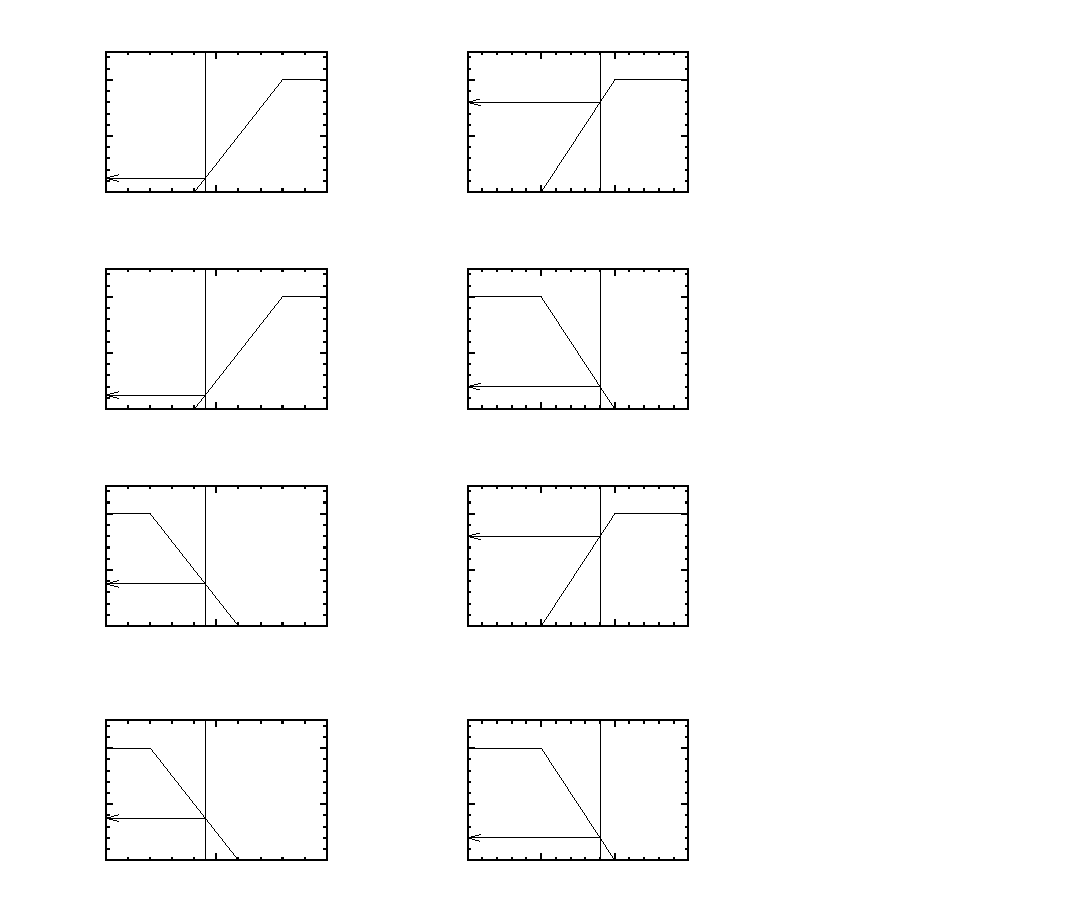
\includegraphics{deduction_of_system_output}}%
    \gplfronttext
  \end{picture}%
\endgroup
